\documentclass{article}


\usepackage[utf8]{inputenc}
\usepackage[czech]{babel}

\usepackage{geometry}
\usepackage{csquotes}

\usepackage{graphicx}
\usepackage{float}

\usepackage{biblatex}
\addbibresource{programmer.bib}


\title{ffteq - Programátorská dokumentace}
\author{Filip Kastl}
\date{\today}

\begin{document}
\maketitle


\section*{Co to je}

Program na upravování 8bit 44,1kHz pcm mono zvukových souborů formátu Wave.
Jeho hlavní součástí je frekvenční zvukový filtr implementovaný pomocí
diskrétní Fourierovy transformace, konkrétně pomocí algoritmu rychlé Fourierovy
transformace. Umí také upravovat hlasitost.

Program byl vyvíjen na Linuxu pomocí \texttt{dotnet core 6.0.301}. Nebyly
použity žádné knihovny vyjma standardních.


\section*{Jak to zkompilovat}

Potřebujete mít nainstalovaný \texttt{dotnet core 6.0}. Pak stačí v kořenovém
adresáři projektu spustit následující příkaz:
\begin{verbatim}
dotnet build -r linux-x64 --no-self-contained
\end{verbatim}
Případně můžete chtít nahradit \texttt{linux-x64} za \texttt{win-x64}. Pokud
chcete, aby byl výsledný program spustitelný i na počítači bez dotnet core 6.0
runtimu, můžete použít command line option \texttt{--self-contained}.
Zkompilované soubory lze najít v \texttt{bin/Debug/net6.0/}.

Je možné kompilovat i pomocí/pro jiné verze dotnet core. Projekt je
kompatibilní i s \texttt{dotnet core 3.1}. V takovém případě je však potřeba
upravit soubor \texttt{ffteq.csproj}.


\section*{Pojmy}

\begin{itemize}
	\item	\textbf{DFT} -- Diskrétní Fourierova transformace. Pro účely
		tohoto programu způsob, jak rozebrat signál na intenzity
		jednotlivých frekvencí.
	\item	\textbf{FFT} -- Konkrétní algoritmus počítající DFT s
		asymptotickou složitostí $O(n \cdot \log{n})$, kde $n$ je délka
		signálu.
	\item	\textbf{sample} -- Analogový zvukový signál je spojitý.
		Digitálně se reprezentuje pomocí pravidelně rozmístěných vzorků
		-- samplů.  Tomuto způsobu zaznamenávání zvukového signálu se
		říká \textbf{PCM} -- Pulse-code modulation.
	\item	\textbf{Wave} -- Jednoduchý formát zvukových souborů. Kóduje
		signál prostě jako pole hodnot samplů.
	\item	\textbf{8bit} -- Jde o označení velikosti jednotlivých samplů.
	\item	\textbf{44,1 kHz, sample rate} -- Jde o rychlost s jakou by
		samply měly být přehrávány.
	\item	\textbf{mono} -- Zvukový signál může být dvoustopý, tedy
		stereo. ffteq se však zabývá pouze jednostopými signály -- mono
		signály.
	\item	\textbf{Low-pass filtr} -- Filtr, který odstraňuje vysoké
		frekvence.
	\item	\textbf{High-pass filtr} -- Filtr, který odstraňuje nízké
		frekvence.
\end{itemize}


\section*{Jak to funguje}

Program načítá a zapisuje Wave soubory pomocí třídy \emph{Wav}. Zvukový signál
je interně reprezentován třídou \emph{Signal}. Více o těchto třídách vizte v
další sekci.

\subsection*{O co se stará která třída}

Soubor \texttt{docs/diagram.pdf} slouží jako přehled tříd a jejich veřejných
memberů. Šipky v diagramu znázorňují vztahy \enquote{třída A spravuje instance
třídy B}.

\subsubsection*{Wav}
Třída zodpovědná za načítání a zapisování Wave souborů. Nepracuje ovšem přímo
se soubory, ale se streamy. Načtení ze streamu probíhá v konstruktoru instance
této třídy. Je zkontrolováno, že hlavička opravdu odpovídá 8bit pcm mono Wave
formátu. Pokud ne, je vyhozena výjimka se zprávou o tom, čím se hlavička liší.
Zápis do streamu se provádí pomocí metody \emph{WriteFile()}.

Načtený signál zpřístupňuje třída skrz property \emph{Signal WavSignal}.

Na konci dokumentu jsou odkazy na hezký přehled formátu souborů
Wave\cite{wav-prehled} a jeho formální specifikaci\cite{wav-spec}.

\subsubsection*{Signal}
Třída, která je interní reprezentací zvukového signálu. Je implementována jako
pole samplů. Každý sample je číslo typu \emph{double} pohybující se od $-1.0$
do $1.0$.

\subsubsection*{Effect}
Abstraktní třída reprezentující efekt aplikovatelný na zvukový signál. Její
jediná veřejná metoda je \emph{Process}, která vezme signál, upraví ho pomocí
efektu a vydá výsledek. Dědí z ní třídy \emph{FFTFilter}, \emph{Gain} a
\emph{Clipping}.

FFTFilter je hlavním efektem programu. Stará se o filtrování signálu. Přes
konstruktor je specifikováno, které frekvence má filtrovat (vizte sekci
filterlo a filterhi v uživatelské dokumentaci). Informace o principu filtru
vizte v sekci Algoritmy.

Gain zvyšuje nebo snižuje hlasitost signálu. Přes konstruktor je specifikován
počet decibelů. Decibely se převadí na poměr amplitud pomocí vzorce $ratio =
\sqrt{10^{db \over 10}}$.

Protože efekty mohou zvýšit hodnotu některých samplů nad $1.0$ nebo snížit pod
$-1.0$, je třeba provést takzvaný clipping signálu. To znamená prostě pro každý
sample provést \linebreak $value = \max(-1.0, \min(1.0, value))$. O clipping se
stará efekt Clipping. Na rozdíl od ostatních efektů, tenhle je aplikován
vždycky a to na konci programu.

\subsubsection*{Windowing}
Informace o principu zpracovávání po oknech vizte v sekci Algoritmy.

Třídy dědící z abstraktní \emph{Windowing} mají za účel zjednodušit
zpracovávání signálu po oknech. Pracuje se s nimi následujícím způsobem:
\begin{enumerate}
	\item	Metodou \emph{StartProcessing()} se předá windowingu vstupní
		signál
	\item	Metoda \emph{NextWindow()} vydá okno vystřižené z původního
		signálu
	\item	Zpracované okno se vrátí windowingu pomocí metody
		\emph{PutBack()}
	\item	Kroky $2$ a $3$ se opakují dokud \emph{NextWindow()} nevrátí
		\emph{null}
	\item	V tu chvíli je hotový výsledný signál a může být vyzvednut
		metodou \emph{FinishProcessing()}
\end{enumerate}
Windowing objekt se sám stará o aplikaci windowing funkce a o překryv.

ffteq obsahuje dvě implementace windowingu. Jednou je \emph{RectWindowing}. To
je triviální implementace bez windowing funkce a bez překryvu. V programu není
použita. Druhou implementací je \emph{HannWindowing} používající Hann windowing
function a překryv $50\%$. To, co je popsané v sekci Algoritmy, odpovídá
chování této třídy.

Windowing používají třídy \emph{CMDOptionFilterLow} a
\emph{CMDOptionFilterHigh}.

\subsubsection*{CMD}
Třídy s předponou CMD se zabývají zpracováváním a vykonáváním argumentů z
příkazové řádky. Vizte uživatelskou dokumentaci pro informace o tom, v jakém
formátu se zadávají terminálové argumenty.

Každá z dostupných options je reprezentována objektem dědícím z abstraktní
třídy \emph{CMDOption}. CMDOption obsahuje \emph{Params} pole objektů dědících
z abstraktní třídy \emph{CMDOptionParam}. Ty reprezentují parametry dané
option. Jejich metoda \emph{Validate()} kontroluje, jestli daný řetězec splňuje
podmínky parametru.

Důležitou metodou objektů dědících z CMDOption je \emph{Execute()}. Skrz ni
option dostane jemu náležící terminálové argumenty a signál a měl by na něm
vykonat svoji funkci. Tedy například \emph{CMDOptionGain} dostane řetězec "-5"
a signálu sníží hlasitost o $5$ decibelů.

V programu dědí z CMDOptionParam pouze \emph{CMDOptionParamDouble}. To je
třída, která kontroluje, že argument je konvertovatelný na C\# typ
\emph{double}. Žádné jiné typy parametrů nebylo třeba implementovat. Kdyby však
program měl být rozšiřován, je určitě možné mít například option s parametrem,
který je validní pouze jako číslo $0$ až $5$ nebo option s parametrem, který je
validní pouze, pokud lze konvertovat na \emph{bool}.

O naparsování seznamu terminálových argumentů na options a validování parametrů
se stará třída \emph{CMDOptionParser}. Ta dostane přes konstruktor pole
CMDOption objektů -- pole options, které program podporuje. Její metoda
\emph{Parse()} pak bere pole terminálových argumentů a vrací pole options a
jejich argumentů v pořadí, v jakém je uživatel zadal na příkazové řádce.

Za jeden běh programu je možná aplikovat stejnou option vícekrát s různými
argumenty.


\subsection*{Algoritmy}

\subsubsection*{FFT}
Rychlá Fourierova transformace je napsána podle pseudokódu v knížce Průvodce
labyrintem algoritmů\cite{pruvodce} na straně 398. Kniha zmiňuje dvě primitivní
$n$-té odmocniny z jedničky pro dané $n$. ffteq používá tu s pozitivní
imaginární složkou.

\subsubsection*{Princip filtrování}
Filtr dostane signál jako seznam samplů. Je to informace o tom, jak se mění
intenzita zvukové vlny v čase. Jako první krok použije DFT, aby se dostal na
jinou reprezentaci signálu -- na informaci o intenzitě jednotlivých frekvencí.
Přejeme si intenzitu některých frekvencí snížit nebo zcela vynulovat. To je v
této reprezentaci snadné. Filtr prostě odpovídající prvky vektoru vynásobí
koeficientem od $0.0$. do $1.0$. Nakonec filtr použije inverzní DFT, aby signál
převedl zpět na seznam samplů.

Je tu ale problém. Od uživatele dostaneme čísla frekvencí, ale DFT nám dá
vektor šířky odpovídající šířce vektoru, který jsme transformovali.
Složkám tohoto vektoru se říká \enquote{bins}. Který bin odpovídá kterým
frekvencím? Na to použijeme následující vzorec:
$$
bin = {{hz \over sample\_rate} \cdot {N}}
$$
kde $N$ je šířka vektoru. Vzorec je adaptovaný z odpovědi na foru Stack
Overflow\cite{overflow}. Nemám potřebné znalosti na to, abych si vzorec odvodil
nebo věděl, v které učebnici ho hledat.

\subsubsection*{Windowing}
Některé efekty není praktické aplikovat na celý signál. V případě tohoto
programu je to \emph{FFTFilter}. Filtr využívá FFT a FFT operuje na vektorech
délky mocniny dvojky. Doplnit každý signál o nuly na další mocninu dvojky by
bylo nejspíš možné a pro účely tohoto programu postačující. Rozhodl jsem se ale
použít zpracování po oknech, protože to je standardní způsob, jak problém
řešit.

Signál je rozsekán na pravidelné úseky -- okna. Efekt se pak aplikuje na každý
úsek zvlášť. Úseky se mohou překrývat. Na úseky je typicky aplikovaná nějaká
window function. Je možné použít okna bez překryvu a bez aplikování window
function. Pak se ale může stát (např. v případě FFT filtru), že na sebe
zpracovaná okna nebudou navazovat. To se manifestuje jako pravidelné cvakání ve
výsledném zvukovém signálu. Abych se mu vyhnul zvolil jsem pro účely FFT filtru
Hann window function a $50\%$ překryv.

Aplikování window function znamená, že každé okno je přenásobeno koeficienty od
$0.0$ do $1.0$, které specifikuje daná funkce. Zde je znázorněno, jak to vypadá
s parametry, které používá ffteq:

\begin{figure}[H]
	\begin{center}
		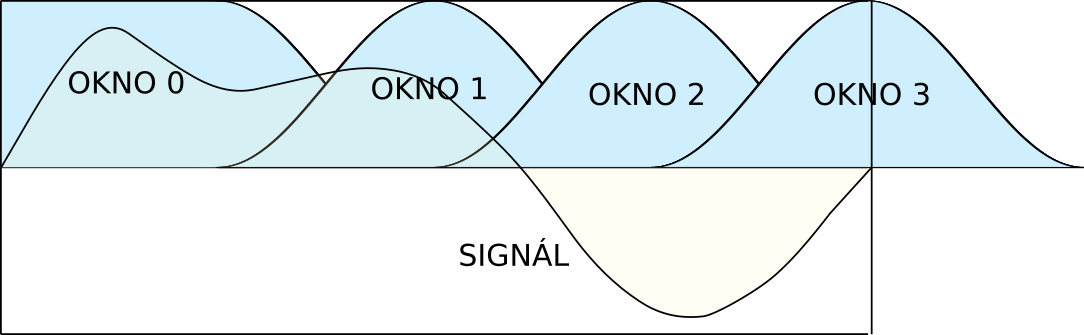
\includegraphics[width=0.6\linewidth]{windowing-1.png}
	\end{center}
\end{figure}

Když jsem vybíral window function, nejprve jsem zkusil naimplementovat
windowing bez window function a bez překryvu. Program nedával uspokojivé
výsledky. Následně jsem vyzkoušel Hann window function, protože to je jedna z
jednodušších na implementaci. Použil jsem $50\%$ překryv, protože s ním se
koeficienty vždy sečtou na $1.0$, jak je vidět na následujícím obrázku:

\begin{figure}[H]
	\begin{center}
		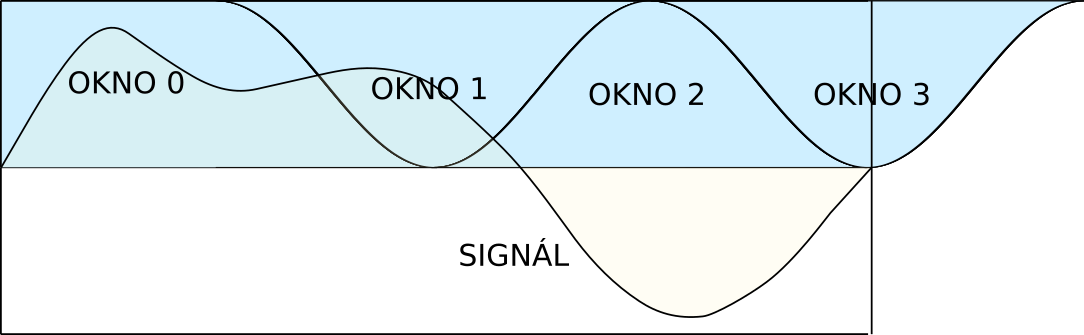
\includegraphics[width=0.6\linewidth]{windowing-2.png}
	\end{center}
\end{figure}

Nemám nijak teoreticky podložené, že toto je správný postup. Pracoval jsem
spíše experimentálně.  Hann window function už dávala uspokojivé výsledky, a
tak jsem u ní zůstal.

Je třeba ošetřit, že první/poslední okno nemají zleva/zprava překryv s žádným
dalším oknem. Já problém řeším tak, že prvnímu oknu dám trošku jiný tvar a na
konec signálu přidám ještě jedno okno přesahující ze signálu ven. Přesah mimo
signál znamená, že okno bude doplněno nulami. Lze se také rozhodnout konce
signálu neošetřovat. Vede to pak k nepatrným náběhům v hlasitosti závislých na
šířce oken.


\section*{Poznámky}

\subsubsection*{Ke zpracovávání terminálových argumentů}
Implementovat vlastní systém parsování terminálových argumentů pravděpodobně
nebylo dobré rozhodnutí. Bylo to časově náročné -- více než jsem očekával.
S výsledkem nejsem spokojený. Systém je funkční, ale myslím si, že by mohl být
méně zmatečný. A hlavně: Pro někoho, kdo můj kód pročítá, by bylo jednodušší
seznámit se s nějakou široce používanou externí knihovnou, než s čímkoliv, co
bych napsal já. Nechť je toto varování pro další programátory, kteří by si
řekli \enquote{Co je na tom, to si zvládnu napsat sám}.


\printbibliography


\end{document}
